\section{Aufbau und Durchführung}
\label{sec:Durchführung}
\subsection{Aufbau}
\subsubsection{Aufbau zur Durchlasskurve}
Um zu untersuchen welchen Frequenzbereich eine LC$_1$C$_2$-Kette durchlässt wird ein Versuchsaufbau nach Abbildung \ref{dfig:1} gewählt.

\begin{figure}[H]
  \centering
  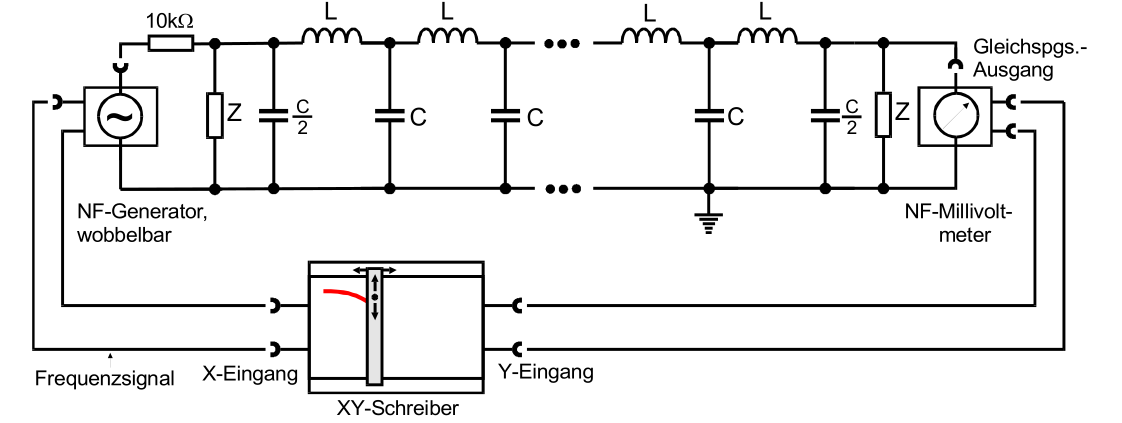
\includegraphics{durchlass.png}
  \caption{Aufbau zur Untersuchung der Durchlasskurve einer LC$_1$C$_2$-Kette.}
  \label{dfig:1}
\end{figure}

Die oben skizzierte LC$_1$C$_2$-Kette besteht im Experiment aus 14 alternierenden LC-Gliedern, bei denen jeweils eine Spule $L$ in Reihe und ein Kondensator, abwechselnd $C_1$ und $C_2$, parallel dazu geschaltet ist.
Die Kette ist am Anfang und am Ende mit dem Wellenwiderstand $Z$ abgeschlossen.
Am Anfang der Kette ist eine Spannungsquelle zugeschaltet.
Der unmittelbar danach geschaltete Widerstand von $\SI{10}{\kilo\ohm}$ dient dazu, den Eigenwiderstand der Spannungsquelle, welche einen systematischen Fehler darstellt, zueleminieren.
Am Ende der LC$_1$C$_2$-Kette befindet sich ein Millivoltmeter, welches die Speisewechselspannung in Gleichspannung umwandelt.
Diese wird dem Y-Eingang eines XY-Schreibers zugeführt, während der X-Eingang mit dem Logarithmus der Speisespannung verbunden wird.
Die LC$_1$C$_2$-Kette hat die Werte
\begin{align*}
  L   &= \SI{1,217}{\milli\henry},\\
  C_1 &= \SI{20,13}{\nano\farad},\\
  C_2 &= \SI{9,41}{\nano\farad},
\end{align*}
wobei der Wellenwiderstand $Z$ noch zu bestimmen ist.
Dieser wird nach Formel (\ref{eqn:irgendwas}) aus der Theorie berechnet und eingestellt.
Er beträgt
\begin{align*}
  Z   &= \SI{999999}{\ohm}.
\end{align*}

\subsubsection{Aufbau zur Dispersionsrelation}
Die Dispersionsrelation wird mit der Schaltung aus Abbildung \ref{dfig:2} untersucht.

\begin{figure}[H]
  \centering
  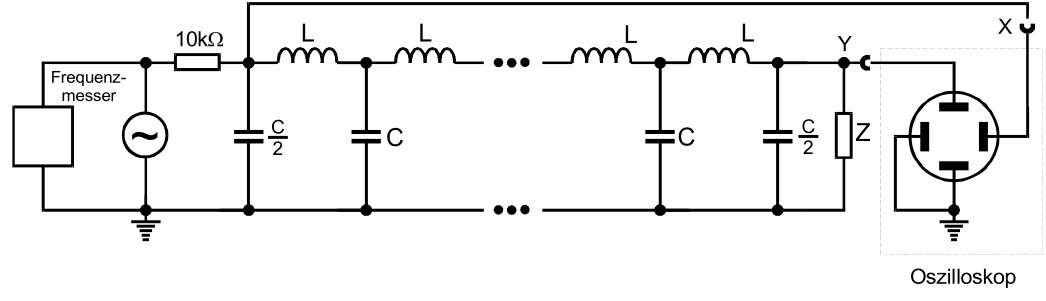
\includegraphics{dispersion.png}
  \caption{Aufbau zur Untersuchung der Dispersionsrelation einer LC$_1$C$_2$-Kette.}
  \label{dfig:2}
\end{figure}

Es handelt sich um eine leicht abgewandelte Schaltung aus Abbildung \ref{dfig:1}.
Das Ende der LC$_1$C$_2$-Kette wird dem Y-Eingang eines Oszilloskops zugeführt.
Der X-Eingang wird mit der Speisespannung verbunden.
Diese ist auch mit einem Frequenzmesser verbunden, da der Anzeige der Spannungsquelle nicht vertraut werden kann.

\subsubsection{Aufbau zur Bestimmung der Eigenfrequenzen und Form der stehenden Wellen}
Hierzu wird die Schaltung aus Abbildung \ref{dfig:2} benutzt.
Jedoch wird an Stelle des Oszilloskops ein Millivoltmeter zugeschaltet.
Zudem soll die Kette für die Bestimmung der Eigenfrequenzen offen sein, was bedeutet, dass der Wellenwiderstand $Z$ überbrückt wird.

\subsection{Durchführung}
\subsubsection{Aufnahme der Durchlasskurve}
Zunächst wird der Wellenwiderstand richtig eingestellt.
Um eine ansehnliche Durchlasskurve aufzunehmen, müssen Spannungsquelle und XY-Schreiber richtig justiert werden.
Die Spannungsquelle wird dabei auf einen kontinuierlichen Frequenzsweep linearer Form eingestellt, während der X- und Y-Eingang des Schreibers entsprechend skaliert wird.
Nach einer langen Friemelei wird die Durchlasskurve über einen einzelnen Sweep aufgenommen.
Gleichzeitig wird die Frequenzskala notiert.
Wichtig beim Aufnehmen ist es, den akustischen und den optischen Ast aufzunehmen.

\subsubsection{Bestimmung der Dispersionsrelation}
Hierzu wird das Oszilloskop auf XY-Betrieb gestellt um die Lissajous-Figuren zu finden, bei denen die Phasenverschiebung $0$ oder $\pi$ ist, sie also eine Gerade ist.
Die Frequenzen, bei denen dies der Fall ist, werden notiert.

\subsubsection{Bestimmung der Eigenfrequenzen}
Hierzu wird wie zuvor vorgegangen.
Diesmal werden aber die Frequenzen notiert, bei denen ein Spannungsmaxima am Ende der Kette beobachtet wird.
Dies sind nämlich die Frequenzen, bei denen sich eine stehende Welle in der Kette bildet.

\subsubsection{Bestimmung der Form der stehenden Wellen}
Um die Form zu bestimmen wird die Frequenz auf die erste bzw. zweite zuvor ermittelte Eigenfrequenz der Kette gestellt.
Es werden die Spannungen pro zugeschaltetem Kettenglied notiert.
Zuletzt wird dasselbe mit einer Eigenfrequenz mit zugeschaltetem Wellenwiderstand durchgeführt.
